\section{Themes}
A \src{DockTheme} relates to \src{DockingFrames} like a \src{LookAndFeel} to \src{Java Swing}. At any given time a \src{DockController} is associated with exactly one theme. The theme defines various graphical elements like icons, painting code and also some behavior. The current \src{DockTheme} can be changed through the method \src{setTheme}:
\begin{lstlisting}
DockController controller = ...
DockTheme theme = new EclipseTheme();
controller.setTheme( theme );
\end{lstlisting}

\subsection{Existing Themes}
Several \src{DockTheme}s are already included in the framework. A list of theme-factories can be accessed through the method \src{getThemes} of \src{DockUI}. This sub-chapter will list up the existing themes and mention some of their specialities.

Keep in mind that \src{DockTheme}s do not have to follow a specific path for setting up their views. All the current themes are derived from \src{BasicTheme} and thus share a lot of concepts. Future or custom themes however might be implemented in different ways.

\subsubsection{NoStackTheme}
This theme is a wrapper around other themes. It prevents \src{StackDockStation}s from having a \src{DockTitle} and makes sure that the user cannot drag or create a \src{StackDockStation} into another \src{StackDockStation}. The code for creating a \src{NoStackTheme} looks like this:
\begin{lstlisting}
DockTheme original = ...
DockTheme theme = new NoStackTheme( original );
\end{lstlisting}

\subsubsection{BasicTheme}
The \src{BasicTheme} is a simple but working theme. All the other themes of the framework build upon \src{BasicTheme}. This theme shows content whenever possible. It tries to use all features and thus is quite good for debugging, to check whether all features are supported.

\begin{figure}[ht]
\centering
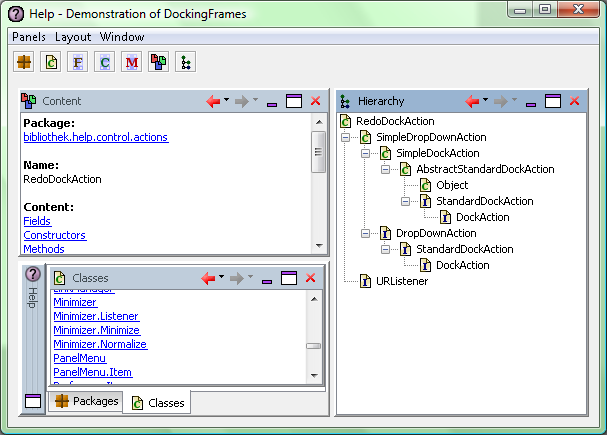
\includegraphics[width=0.5\textwidth]{themes/theme_default}
\caption{BasicTheme}
\label{fig:theme_flat}
\end{figure}

\subsubsection{SmoothTheme}
\src{SmoothTheme} is basically the same as \src{BasicTheme}. The only difference is a replaced default-\src{DockTitleFactory}. As a result new \src{DockTitle}s are used by most elements, these new titles smoothly change their color when the ``active'' state of their \src{Dockable}s changes.

\subsubsection{FlatTheme}
\src{FlatTheme} is a variation of \src{BasicTheme} that tries to minimze the number of borders. Among other things it uses new \src{DockTitle}s and new views for \src{DockAction}s. It is the ideal theme for developers that want to learn how to customize an existing theme.

\begin{figure}[ht]
\centering
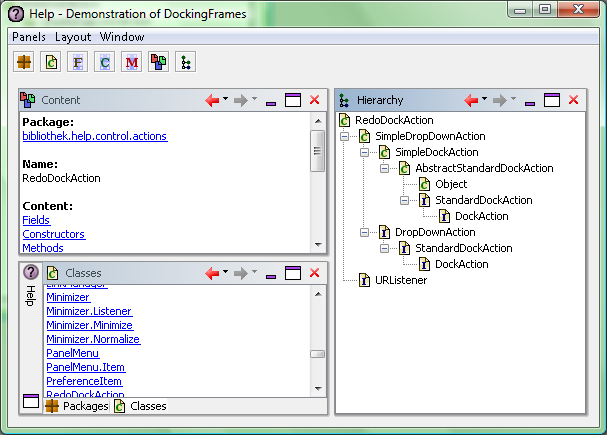
\includegraphics[width=0.5\textwidth]{themes/theme_flat}
\caption{FlatTheme}
\label{fig:theme_basic}
\end{figure}

\subsubsection{BubbleTheme}
A more experimental theme. \src{BubbleTheme} often uses animations and other graphical gimmicks. It has a few performance issues, but it is a good theme to demonstrate the potential of the theme-mechanisms.

\begin{figure}[ht]
\centering
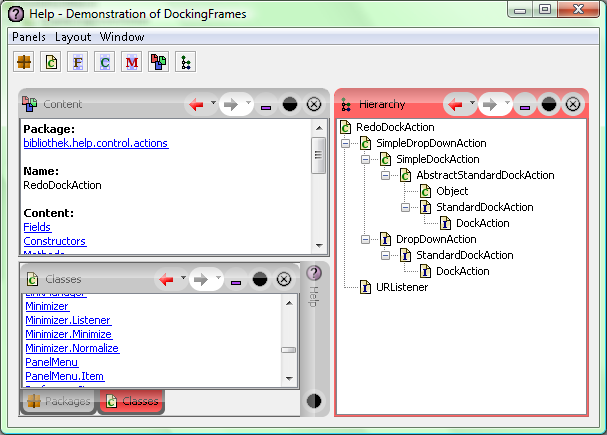
\includegraphics[width=0.5\textwidth]{themes/theme_bubble}
\caption{BubbleTheme}
\label{fig:theme_bubble}
\end{figure}

\subsubsection{EclipseTheme}
\src{EclipseTheme} tries to mimmic the behavior and look of the well known IDE Eclipse. All the \src{Dockable}s are shown on tabbed-components and often \linebreak \src{DockTitle}s are replaced by the tabs. The theme does not use the default theme-mechanisms as often as other themes and it might be a bit tricky to customize the theme. On the other hand it certainly looks good.

\begin{figure}[ht]
\centering
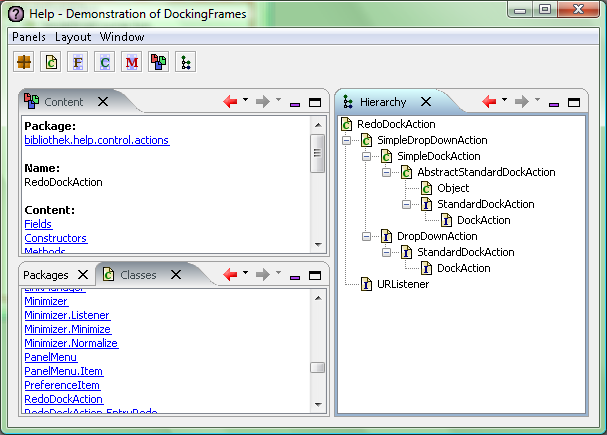
\includegraphics[width=0.5\textwidth]{themes/theme_eclipse}
\caption{EclipseTheme}
\label{fig:theme_eclipse}
\end{figure}

\src{EclipseTheme} offers some keys the map of properties that is stored in \src{DockProperties}. The keys are:
\begin{description}
	\item[PAINT\_ICONS\_WHEN\_DESELECTED] A \src{Boolean} that tells whether \linebreak icons on tabs should be painted if the tab is not selected. In every tabbed-component one tab has to be selected and its associated \src{Dockable} is the only visible element on the component.
	\item[THEME\_CONNECTOR] An \src{EclipseThemeConnector}. The connected tells whether a \src{DockAction} belongs onto a tab, or in a separate list of ``unimportant'' actions. The connector also tells what kind of title to use for a \src{Dockable}.
	\item[TAB\_PAINTER] A \src{TabPainter}. This class is a factory that creates the tab-components and sets up other settings that are related with tabs.
\end{description}

\classbox{The \src{DefaultEclipseThemeConnector} puts every \src{DockAction} which is annotated with \src{EclipseTabDockAction} onto tabs.}

\warningbox{The settings for titles and borders that are given by an \src{EclipseThemeConnector} are not respected if the element is on a \src{StackDockStation}s. A \src{StackDockStation} always uses some tabbed-component.}


\subsection{Custom Theme}
With the exception of the classes that are directly related to a \src{DockTheme} no code in the framework depends on a special undocummented behavior of a theme. Clients can reimplement the interface \src{DockTheme} without fear to break things.

A better approach then full reimplementation might be to extend the class \src{BasicTheme}. This class provides some default values which can easily be \linebreak changed by the appropriate \src{setXZY} method.

\src{DockTheme} has a method \src{install}, this method can be used to exchange some values that are not stored in the \src{DockTheme} itself. For example to exchange icons in the \src{IconManager}.

\warningbox{A theme dives deep into the framework. Implementing a new theme requires a lot of time and a good understanding of the framework. This document might help to understand the basics, but some stuff can only be found out by looking directly at the source code.}

\subsection{Customizing}
More than 50\% of the frameworks source code is only used for painting stuff. No \src{DockTheme} uses particular complex code, just the mass can lead to some loss of direction. This sub-chapter will give only an overview of the basic classes, interfaces and concepts.

\infobox{Many of the mechanisms used by \src{DockTheme}s can be used by clients as well.}

\subsubsection{UI-Properties} \label{sec:uiproperties}
The \src{UIProperties} distribute properties like colors, texts or fonts in the framework. The basic idea is to use a map. The keys are \src{String}s, the values are the properties. A \src{DockTheme} or a client can modify or put new key-value pairs into the map and components can read those values which are interesting for them.

While \src{UIProperties} build upon a map, they can do more than an ordinary map. They report changes in the map through an observer mechanism represented by \src{UIValue}s. Further more they can filter their content through \src{UIBridge}s.

The full list of classes and interfaces building the base for the UI-properties consists of:
\begin{itemize}
	\item \src{UIProperties}: The map that connects properties, observers and filters.
	\item \src{V}: The type of the properties, e.g. the class \src{Color}.
	\item \src{UIValue}: An observer that is attached to \src{UIProperties} and receives an event if a property changes. The \src{UIValue} has to provide information to the filters, that means an \src{UIValue} represents the component that is using the property.
	\item \src{UIBridge}: An \src{UIBridge} is a filter between the \src{UIProperties} and the \src{UIValue}s. An \src{UIBridge} can decide to inform an \src{UIValue} about a changed property at any time. Depending on the target \src{UIValue} an \src{UIBridge} may filter the property in different ways.
	\item{UIScheme}: a set of default properties and default \src{UIBridges}.
\end{itemize}

The implementation gets more complex:
\begin{itemize}
	\item For each key several \src{V} properties can be put into the map. Each value gets assigned another priority (``default'', ``theme'' or ``client'') and only the one with the highest priority is used.
	\item Each \src{UIValue} is associated with a \src{Path}. The \src{Path} tells what type the \src{UIValue} has.
	\item \src{UIBridge}s are also associated with a \src{Path}. An \src{UIBridge} is responsible to handle all those \src{UIValue}s that are associated either with the same \src{Path} or a \src{Path} that has the bridges \src{Path} as prefix.
\end{itemize}

\designbox{This scheme allows a flexible handling of resources. On one hand the number of keys is limited and one method call is enough to change a lot things in the user interface (e.g. all background colors of titles). On the other hand clients can implement sophisticated strategies to change some properties without the need to know in detail how the property will be used.

Originally this mechanism was invented to handle \src{Color}s. Then it became evident that the same mechanism could be used for other resources as well. The current implementation requires to implement several classes for each type of resource. While this might be annoying for the first use it ensures type safety. In a system where cause (writing in the map) and effect (reading from the map) can be separated by dozens of classes and an unknown amount of time one does not want to care about types as well.}

There are several subclasses of \src{UIProperties}, each of these classes handles another kind of property:
\begin{itemize}
 \item \src{ColorManager} handles \src{Color}s.
 \item \src{FontManager} handles \src{Font}s. Rather than distributing \src{Font}s directly, this class distributes \src{FontModifiers}. A \src{FontModifier} can use the default font of a component slightly modify it (e.g. make it italic), or just replace the font.
 \item \src{IconManager} handles \src{Icon}s.
 \item \src{TextManager} handles language dependent text.
 \item \src{ThemeManager} is not directly a subclass, but offers a similar interface. It is responsible for distributing factories and strategies used all over the framework.
\end{itemize}

\subsubsection{Colors}
In order to understand this chapter \ref{sec:uiproperties} should be read first.

All the colors used in the framework are handled by the \src{ColorManager}. The \src{ColorManager} is an \src{UIProperties} and can be accessed through the \linebreak \src{DockController}. It's use could look like this:
\begin{lstlisting}
DockController controller = ...
ColorManager colors = controller.getColors();
colors.put( Priority.CLIENT, "title.active.left", Color.GREEN );
\end{lstlisting}
In this snippet the value for the key ``title.active.left'' is changed to green. The priority \src{CLIENT} is highest possible priority. It is never overridden by the framework.

Or a more sophisticated use could involve a \src{ColorBridge}:
\begin{lstlisting}
DockController controller = ...
ColorManager colors = controller.getColors();
colors.publish( Priority.CLIENT, TitleColor.KIND_TITLE_COLOR, new ColorBridge(){
	public void add( String id, DockColor uiValue ){
		// ignore
	}
	public void remove( String id, DockColor uiValue ){
		// ignore
	}
	public void set( String id, Color value, DockColor uiValue ){
		TitleColor title = (TitleColor)uiValue;
		if( title.getTitle().getDockable() == <somevalue> )
			title.set( Color.GREEN );
		else
			title.set( value );
	}	
});
\end{lstlisting}
Here a \src{ColorBridge} for the \src{Path} \src{KIND\_TITLE\_COLOR} is installed in line \src{3}. This path is only used by \src{UIValue}s that implement \src{TitleColor}. Hence the unchecked cast from \src{DockColor} to \src{TitleColor} in line \src{11} is safe. The methods \src{add} (line \src{4-6}) and \src{remove} (line \src{7-9}) are called by \src{UIProperties} when a \src{UIValue} gets added or removed to it. These methods can be ignored as long as the bridge does not change the color on its own. Otherwise the \src{DockColor}s could be stored in some list and their method \src{set} could be called whenever the color needs to be exchanged.

This bridge searches for a specific \src{Dockable} called ``somevalue'' (line \src{12}). The bridge returns \src{GREEN} for all colors used by any title of this \src{Dockable}. There is no distinction between the colors for background, foreground or other usages.

\codebox{An example showing the same things as the snippets is ``UI Properties: Color''}

\infobox{There is no global list of keys and every \src{DockTheme} uses different keys. All the modules that need colors are annotated with \src{ColorCodes} and expose their own list of keys to the API-documentation. Also the various implementations of \src{ColorScheme} can be used to find keys.}

\classbox{All the standard themes use a \src{ColorScheme} as their initial set of colors. All the standard themes provide a key for the \src{DockProperties} to change that initial scheme. For example the key provided by \src{BasicTheme} is stored as constant \src{BASIC\_COLOR\_SCHEME}. There are several subclasses of \src{ColorScheme} for the different themes.}

By the way: some themes use colors that are read from the current \linebreak \src{LookAndFeel}. Clients can call the method \src{registerColors} of \src{DockUI}. This method takes a \src{LookAndFeelColors} which is responsible in reading the colors from the \src{LookAndFeel}.

\subsubsection{Fonts}
Fonts use the same mechanism as Colors. A \src{FontManager} can be accessed through the methods \src{getFonts} of \src{DockController}. Unlike colors a set of standard keys are defined as constants in \src{DockFont}.

The \src{FontManager} does not distribute \src{Font}-objects but \src{FontModifier}s. A \src{FontModifier} has one method that receives the original \src{Font} and can return any \src{Font} it likes. In example a \src{FontModifier} could inverse the bold-property of a \src{Font}. There are two \src{FontModifiers} ready to use:
\begin{itemize}
	\item \src{ConstantFontModifier} does not modify anything but always return the same \src{Font}
	\item \src{GenericFontModifier} can modify the italic-, bold- and size-property of a font.
\end{itemize}

\classbox{Clients that want to use a \src{FontModifier} might be interested in the classes \src{DLabel} and \src{DPanel} which already modify their font. Also the class \src{FontUpdater} can be used to create new \src{JComponent}s with the capability to modify their font.}

\subsubsection{Icons}
\src{Icon}s can be modified through the \src{IconManager}. The \src{IconManager} can be accessed through the method \src{getIcons} of \src{DockController}. It is an \linebreak \src{UIProperties} and offers all the methods that are known from colors and fonts.

There is no global list of keys in the source code. However the file ``icons.ini'' contains a list of keys and paths of all the default icons.

\subsubsection{Text}
Language dependend text is distributed by the \src{TextManager}, it can be accessed through \src{DockController.getTexts()}. The \src{TextManager} is an \src{UIProperties} and offers all the methods that are known from colors and fonts.

The default text for different languages is stored in several \src{*.properties} files. These files can be loaded by \src{ResourceBundle}s. Clients can make use of the class \src{DefaultTextScheme} to load additional languages into the framework.

\subsubsection{Actions}
The views for \src{DockAction}s are changed through the \src{ActionViewConverter}. Please read chapter \ref{sec:actions} for more information.

\subsubsection{Titles}
\src{DockTitle}s are managed by the \src{DockTitleManager}. Please read chapter \ref{sec:titles} for more information.

\subsubsection{Border}
Any \src{Border} can be modified or replaced by a \src{BorderModifier}. 

\src{BorderModifier}s can be set by the \src{ThemeManager}. The \src{BorderModifier} interface works in the same way as the \src{FontModifier} interface.

\subsubsection{Background}
The usual background of a \src{Component} is either grey or transparent. Clients can set a painting algorithm for the background with help of the interface \src{BackgroundPaint}. Instances of \src{BackgroundPaint} are applied through the \src{ThemeManager}.

The method \src{paint} of \src{BackgroundPaint} is called every time when a component has to be repainted. The method receives a \src{PaintableComponent} which offers the standard algorithms to paint border, children and other stuff. The \src{BackgroundPaint} can freely decide what to paint and in which order to paint.

\subsubsection{Drag and drop decorations}
During drag and drop operations \src{DockStation}s use a \src{StationPaint} to paint decorations. The \src{StationPaint} can be set through the \src{ThemeManager}.

\subsubsection{Displayers}
A \src{DockableDisplayer} is a wrapper around a \src{Dockable} painting some decorations like a title or some border. All \src{DockStation}s make use of \linebreak \src{DockableDisplayer}s to paint their children. \src{DockableDisplayer}s are created by \src{DisplayerFactory}s which are accessible through the \src{ThemeManager}.

Once a \src{DockableDisplayer} is created it cannot be replaced until either the theme is exchanged or the displayer marks itself as invalid. In the later case the displayer needs to call the \src{discard} method of any \src{DockableDisplayerListener} that was added to it.

Clients are free to implement new displayers or extend existing displayers. Any new displayer should be a focus-cycle-root, assuming the displayer uses \src{Swing}-components the code below can be used to setup the correct focus management:
\begin{lstlisting}
// the new displayer
DockableDisplayer displayer = ...

JComponent root = (JComponent)displayer.getComponent();

root.setFocusable( true );
root.setFocusCycleRoot( true );
root.setFocusTraversalPolicy( 
	new DockFocusTraversalPolicy( 
		new DisplayerFocusTraversalPolicy( displayer ), true ));
\end{lstlisting}